% ------------------------------------------------------
% ------------------------------------------------------------------------
% abnTeX2: Modelo de Trabalho Academico (tese de doutorado, dissertacao de
% mestrado e trabalhos monograficos em geral) em conformidade com 
% ABNT NBR 14724:2011: Informacao e documentacao - Trabalhos academicos -
% Apresentacao
% ------------------------------------------------------------------------
% ------------------------------------------------------------------------

\documentclass[
	% -- opções da classe memoir --
	12pt,				% tamanho da fonte
	openright,			% capítulos começam em pág ímpar (insere página vazia caso preciso)
	twoside,			% para impressão em verso e anverso. Oposto a oneside
	a4paper,			% tamanho do papel. 
	% -- opções da classe abntex2 --
	chapter=TITLE,		% títulos de capítulos convertidos em letras maiúsculas
	%section=TITLE,		% títulos de seções convertidos em letras maiúsculas
	%subsection=TITLE,	% títulos de subseções convertidos em letras maiúsculas
	%subsubsection=TITLE,% títulos de subsubseções convertidos em letras maiúsculas
	% -- opções do pacote babel --
	english,			% idioma adicional para hifenização
	brazil				% o último idioma é o principal do documento
	]{abntex2}

% ---
% Pacotes básicos 
% ---
\usepackage{lmodern}			% Usa a fonte Latin Modern			
\usepackage[T1]{fontenc}		% Selecao de codigos de fonte.
\usepackage[utf8]{inputenc}		% Codificacao do documento (conversão automática dos acentos)
\usepackage{lastpage}			% Usado pela Ficha catalográfica
\usepackage{indentfirst}		% Indenta o primeiro parágrafo de cada seção.
\usepackage{color}				% Controle das cores
\usepackage{graphicx}			% Inclusão de gráficos
\usepackage{microtype} 			% para melhorias de justificação
\usepackage{hyperref}
\usepackage{trivfloat}
\usepackage{datetime}
\usepackage{graphicx}


%\usepackage{listings} usado pra colocar codigo


\trivfloat{quadro}





\usepackage{novacapa}
% ---
		
% ---
% Pacotes adicionais, usados apenas no âmbito do Modelo Canônico do abnteX2
% ---
%\usepackage{lipsum}				% para geração de dummy text
% ---

% ---
% Pacotes de citações
% ---
\usepackage[brazilian,hyperpageref]{backref}	 % Paginas com as citações na bibl
\usepackage[alf]{abntex2cite}	% Citações padrão ABNT

% --- 
% CONFIGURAÇÕES DE PACOTES
% --- 

% ---
% Configurações do pacote backref
% Usado sem a opção hyperpageref de backref
\renewcommand{\backrefpagesname}{Citado na(s) página(s):~}
% Texto padrão antes do número das páginas
\renewcommand{\backref}{}
% Define os textos da citação
\renewcommand*{\backrefalt}[4]{
	\ifcase #1 %
		Nenhuma citação no texto.%
	\or
		Citado na página #2.%
	\else
		Citado #1 vezes nas páginas #2.%
	\fi}%
% ---

% ---
% Informações de dados para CAPA e FOLHA DE ROSTO
% ---
\titulo{Thin Client: Com Raspberry PI}
\autor{Felipe Lima Morais}
\local{Dourados, MS}
\data{2015}
\orientador{Prof. Dr. Fabrício Sérgio de Paula}
\instituicao{Universidade Estadual de Mato Grosso do Sul}


\tipotrabalho{Trabalho de Conclusão de Curso em Ciência da Computação}
% O preambulo deve conter o tipo do trabalho, o objetivo, 
% o nome da instituição e a área de concentração 
\preambulo{Este  exemplar  corresponde  à  redação  finalda
monografia da disciplina Projeto Final de
Curso devidamente corrigida e defendida
por \imprimirautor \  e aprovada pela
Banca  Examinadora, como parte dos
requisitos para a obtenção do título de
Bacharel em Ciência da Computação.}
% ---


% ---
% Configurações de aparência do PDF final

% alterando o aspecto da cor azul
\definecolor{blue}{RGB}{41,5,195}
%\definecolor{blue}{RGB}{0,0,0}

% informações do PDF
\makeatletter
\hypersetup{
     	%pagebackref=true,
		pdftitle={\@title}, 
		pdfauthor={\@author},
    	pdfsubject={\imprimirpreambulo},
	    pdfcreator={LaTeX with abnTeX2},
		pdfkeywords={abnt}{latex}{abntex}{abntex2}{trabalho acadêmico}, 
		colorlinks=false,       		% false: boxed links; true: colored links
    	linkcolor=blue,          	% color of internal links
    	citecolor=blue,        		% color of links to bibliography
    	filecolor=magenta,      		% color of file links
		urlcolor=blue,
		bookmarksdepth=4
}
\makeatother
% --- 

% --- 
% Espaçamentos entre linhas e parágrafos 
% --- 

% O tamanho do parágrafo é dado por:
\setlength{\parindent}{1.3cm}

% Controle do espaçamento entre um parágrafo e outro:
\setlength{\parskip}{0.2cm}  % tente também \onelineskip



\renewcommand{\imprimircapa}{%     CAPA MODELO DE CIÊNCIA DA COMPUTAÇÂO
\begin{capa}%
	\center
	

	\begin{tabular}{@{}c@{}}
	\toprule
	Curso de Ciência da Computação            \\
	\ \ \ \ \ \ \ \ \ \ \ \ \ \ \ \ \ Universidade Estadual de Mato Grosso do Sul\ \ \ \ \ \ \ \ \ \ \ \ \ \ \ \ \  \\ \bottomrule
	\end{tabular}

	
	
	
	\vspace*{\fill}
	\begin{center}
		\ABNTEXchapterfont\bfseries\LARGE\imprimirtitulo
	\end{center}

	\vspace*{\fill} 
	{\large \imprimirautor}
	\\
	\vspace*{\fill}
	\imprimirorientador
	\\
	\vspace*{\fill}
	{\large Curso de Ciência da Computação}
	
	Universidade Estadual de Mato Grosso do Sul
	\\
	\vspace*{\fill}
	
	\large\imprimirlocal \\
	\large\imprimirdata
	\vspace*{1cm}
	
\end{capa}
}



\makeatletter
\renewcommand{\folhaderostocontent}{
\begin{center}
{\ABNTEXchapterfont\bfseries\Large\imprimirtitulo}
\vspace*{\fill}\vspace*{\fill}
\begin{center}
\Large\imprimirautor
\end{center}
\vspace*{\fill}
\abntex@ifnotempty{\imprimirpreambulo}{%
\hspace{.45\textwidth}
\begin{minipage}{.5\textwidth}
\imprimirpreambulo \\
\end{minipage}%
\vspace*{\fill}
}%


\abntex@ifnotempty{\imprimirpreambulo}{%
\hspace{.45\textwidth}
\begin{minipage}{.5\textwidth}
	\begin{center}	
	Dourados, \today \\
	\end{center}
	\vspace*{2cm}
	\begin{center}	
	\imprimirorientador \\
	\end{center}
\end{minipage}%
\vspace*{\fill}
}%



\vspace*{1cm}
\end{center}
}
\makeatother






% ---
% compila o indice
% ---
\makeindex
% ---

% ----
% Início do documento
% ----
\begin{document}

% Seleciona o idioma do documento (conforme pacotes do babel)
%\selectlanguage{english}
\selectlanguage{brazil}

% Retira espaço extra obsoleto entre as frases.
\frenchspacing 

% ----------------------------------------------------------
% ELEMENTOS PRÉ-TEXTUAIS
% ----------------------------------------------------------
% \pretextual

% ---
% Capa
% ---
\imprimircapa %default antex2 





% ---

% ---
% Folha de ros
% (o * indica que haverá a ficha bibliográfica)
% ---
\imprimirfolhaderosto*
% ---

% ------------------------------------------------------------------------------------------------------------
% Inserir a ficha bibliografica
% -----------------------------------------------------------------------------------------------------------

% Isto é um exemplo de Ficha Catalográfica, ou ``Dados internacionais de
% catalogação-na-publicação''. Você pode utilizar este modelo como referência. 
% Porém, provavelmente a biblioteca da sua universidade lhe fornecerá um PDF
% com a ficha catalográfica definitiva após a defesa do trabalho. Quando estiver
% com o documento, salve-o como PDF no diretório do seu projeto e substitua todo
% o conteúdo de implementação deste arquivo pelo comando abaixo:
%
% \begin{fichacatalografica}
%     \includepdf{fig_ficha_catalografica.pdf}
% \end{fichacatalografica}

% 																Area comentada 
%\begin{fichacatalografica}
%	\sffamily
%	\vspace*{\fill}					% Posição vertical
%	\begin{center}					% Minipage Centralizado
%	\fbox{\begin{minipage}[c][8cm]{13.5cm}		% Largura
%	\small
%	MORAIS, Felipe Lima.
%	%Sobrenome, Nome do autor
%	
%	\hspace{0.5cm} \imprimirtitulo. \\
%
%	\hspace{0.5cm} \parbox[t]{\textwidth}{\imprimirtipotrabalho. \imprimirlocal. \\
%	\imprimirinstituicao, \imprimirdata.}\\
%	
%	\hspace{8.75cm} CDD: 02:141:005.7\\
%	\end{minipage}}
%	\end{center}
%\end{fichacatalografica}



% -----------------------------------------------------------------------------------------------------------
% Fim ficha bibliografica
% -----------------------------------------------------------------------------------------------------------



% -----------------------------------------------------------------------------------------------------------
% Inserir folha de aprovação
% -----------------------------------------------------------------------------------------------------------

% Isto é um exemplo de Folha de aprovação, elemento obrigatório da NBR
% 14724/2011 (seção 4.2.1.3). Você pode utilizar este modelo até a aprovação
% do trabalho. Após isso, substitua todo o conteúdo deste arquivo por uma
% imagem da página assinada pela banca com o comando abaixo:
%
% \includepdf{folhadeaprovacao_final.pdf}
%

%																	Area comentada
%\begin{folhadeaprovacao}
%
%  \begin{center}
%    {\ABNTEXchapterfont\large\imprimirautor}
%
%    \vspace*{\fill}\vspace*{\fill}
%    \begin{center}
%      \ABNTEXchapterfont\bfseries\Large\imprimirtitulo
%    \end{center}
%    \vspace*{\fill}
%    
%    \hspace{.45\textwidth}
%    \begin{minipage}{.5\textwidth}
%        \imprimirpreambulo
%    \end{minipage}%
%    \vspace*{\fill}
%   \end{center}
%        
%   Trabalho aprovado. \imprimirlocal, \imprimirdata:
%
%   \assinatura{\textbf{\imprimirorientador} \\ Orientador} 
%   \assinatura{\textbf{Professor} \\ Convidado 1}
%   \assinatura{\textbf{Professor} \\ Convidado 2}
%      
%   \begin{center}
%    \vspace*{0.5cm}
%    {\large\imprimirlocal}
%    \par
%    {\large\imprimirdata}
%    \vspace*{1cm}
%  \end{center}
%  
%\end{folhadeaprovacao}

% -----------------------------------------------------------------------------------------------------------
% Fim folha de aprovação
% -----------------------------------------------------------------------------------------------------------



% -----------------------------------------------------------------------------------------------------------
% Dedicatória
% -----------------------------------------------------------------------------------------------------------

%\begin{dedicatoria}
%   \vspace*{\fill}
%   \centering
%   \noindent
%   \textit{DEDICATORIA PRA QUEM QUISER} \vspace*{\fill} %TODO
%\end{dedicatoria}

% -----------------------------------------------------------------------------------------------------------
% Fim Dedicatória
% -----------------------------------------------------------------------------------------------------------



% -----------------------------------------------------------------------------------------------------------
% Agradecimentos
% -----------------------------------------------------------------------------------------------------------

%\begin{agradecimentos}
%Os agradecimentos principais são direcionados à mim. %TODO
%\end{agradecimentos}

% -----------------------------------------------------------------------------------------------------------
% Fim Agradecimentos
% -----------------------------------------------------------------------------------------------------------



% -----------------------------------------------------------------------------------------------------------
% Epígrafe
% -----------------------------------------------------------------------------------------------------------

%\begin{epigrafe}
%    \vspace*{\fill}
%	\begin{flushright}
%		\textit{"Não vos amoldeis às estruturas deste mundo, \\
%		mas transformai-vos pela renovação da mente, \\
%		a fim de distinguir qual é a vontade de Deus: \\
%		o que é bom, o que Lhe é agradável, o que é perfeito."\\
%		(Bíblia Sagrada, Romanos 12, 2)}
%	\end{flushright}
%\end{epigrafe}

% -----------------------------------------------------------------------------------------------------------
% Fim Epígrafe
% -----------------------------------------------------------------------------------------------------------



% -----------------------------------------------------------------------------------------------------------
% Resumos
% -----------------------------------------------------------------------------------------------------------

% resumo em português
\setlength{\absparsep}{18pt} % ajusta o espaçamento dos parágrafos do resumo
\begin{resumo}
Este trabalho realiza um estudo sobre o uso do Raspberry PI com Thin Client/cliente magro. O Raspberry PI é um computador do tamanho de um cartão de credito que foi desenvolvido para....

(TERMINAR ....)


 \textbf{Palavras-chave}: Conexão Cliente/Servidor. Linux. Rede Local.	%TODO
\end{resumo}

% resumo em inglês
\begin{resumo}[Abstract]
 \begin{otherlanguage*}{english}
   Thin client is a system of low cost, for access, the computers.

   \vspace{\onelineskip}
 
   \noindent 
   \textbf{Keywords}: conection client/server. Linux. LAN.
 \end{otherlanguage*}
\end{resumo}

% -----------------------------------------------------------------------------------------------------------
% Fim Resumos
% -----------------------------------------------------------------------------------------------------------



% -----------------------------------------------------------------------------------------------------------
% inserir o súmario
% -----------------------------------------------------------------------------------------------------------

\pdfbookmark[0]{\contentsname}{toc}
\tableofcontents*
\cleardoublepage

% -----------------------------------------------------------------------------------------------------------
% Fim súmario
% -----------------------------------------------------------------------------------------------------------



% -----------------------------------------------------------------------------------------------------------
% inserir lista de ilustrações
% -----------------------------------------------------------------------------------------------------------

\pdfbookmark[0]{\listfigurename}{lof}
\listoffigures*
\cleardoublepage

% -----------------------------------------------------------------------------------------------------------
% Fim lista de ilustrações
% -----------------------------------------------------------------------------------------------------------



% -----------------------------------------------------------------------------------------------------------
% inserir lista de tabelas
% -----------------------------------------------------------------------------------------------------------

\pdfbookmark[0]{\listtablename}{lot}
\listoftables*
\cleardoublepage

% -----------------------------------------------------------------------------------------------------------
% Fim lista de tabelas
% -----------------------------------------------------------------------------------------------------------



% -----------------------------------------------------------------------------------------------------------
% inserir lista de abreviaturas e siglas
% -----------------------------------------------------------------------------------------------------------

\begin{siglas}						
  %\item[TCP] Transmission Control Protocol - Protocolo de Controle de Transmissão
  %\item[IP] Internet Protocol - Protocolo de Internet
  %\item[TCP/IP]  Conjunto de protocolos usados em redes de computadores
  \item[I/O] Input/Onput
  %\item[LAN] local area network - Rede de área local
  \item[PC] Personal Computer
  \item[GNU] GNU is Not Unix
  \item[CD-ROM] Compact Disc Read-Only Memory
  \item[CD] Compact Disc
  \item[DHCP] Dynamic Host Configuration Protocol
  \item[TFTP] Trivial File Transfer Protocol 
  \item[XDMCP] X Display Manager Control Protocol
  \item[LTSP] Linux Terminal Server Project
  \item[DRBL] Diskless Remote Boot in Linux
  \item[RDP] Remote Desktop Protocol
  \item[PXE] Preboot eXecution Environment
  \item[HD] Hard Disc
  \item[USB] Universal Serial Bus
  \item[RAM] Random Access Memory
  \item[HDMI] High-Definition Multimedia Interface
  \item[VGA] Video Graphics Array
  \item[DDR3] Double Data Rate tipo 3
  \item[DVI-I] Digital Visual Interface (digital e analógico)
  \item[RJ-45] Registered Jack tipo 45
  \item[TI] Tecnologia da Informação
  \item[ARM] Advanced RISC Machine
  \item[MB] MegaByte 
  \item[mA] miliAmpère
  \item[SD] Secure Digital
  \item[NTSC] National Television System Committee
  \item[PAL] Phase Alternating Line
  \item[GPIO] General Purpose Input/Output
  \item[MHz] MegaHertz
  \item[GHz] GigaHertz
  \item[RCA] Radio Corporation of America
  \item[LCD] liquid crystal display
  \item[GPU] Graphics Processing Unit
  \item[GIF] Graphics Interchange Format
  \item[DSLR] digital single-lens reflex 
  \item[NFS] Network File System
  \item[NIS] Network Information Service

\end{siglas}

% -----------------------------------------------------------------------------------------------------------
% Fim lista de abreviaturas e siglas
% -----------------------------------------------------------------------------------------------------------



% -----------------------------------------------------------------------------------------------------------
% inserir lista de símbolos
% -----------------------------------------------------------------------------------------------------------

%\begin{simbolos}						%TODO
%  \item[$ \Gamma $] Letra grega Gama
%  \item[$ \Lambda $] Lambda
%  \item[$ \zeta $] Letra grega minúscula zeta
%  \item[$ \in $] Pertence
%\end{simbolos}

% -----------------------------------------------------------------------------------------------------------
% Fim lista de símbolos
% -----------------------------------------------------------------------------------------------------------



% ----------------------------------------------------------
% ELEMENTOS TEXTUAIS
% ----------------------------------------------------------
\textual



% -----------------------------------------------------------------------------------------------------------
% Introdução (exemplo de capítulo sem numeração, mas presente no Sumário)
% -----------------------------------------------------------------------------------------------------------




% -----------------------------------------------------------------------------------------------------------
% Fim Introdução
% -----------------------------------------------------------------------------------------------------------



% -----------------------------------------------------------------------------------------------------------
% Capitulo de revisão de literatura
% -----------------------------------------------------------------------------------------------------------

\part{Referencial Teórico}

\chapter{thin client}

\section{O que é?}

O thin client, ou cliente magro (tradução literal) é um computador cliente em uma rede  com paradigma de computação centralizada (cliente-servidor), no qual tem poucos ou nenhum aplicativo instalado, sendo totalmente dependente do servidor. O servidor executa programas e armazena dados para seus clientes/thin clients, facilitando o backup e a atualização desse programas, além de compartilhar os recursos de hardware como disco rigido, Mermoria RAM, CPU, entre outros\cite{ComoFuncionaThinClient, tanenbaum2010sistemas}.

Existe também aparelhos de thin client que são equipamentos similares a computadores pessoais ou PCs. O que difere esses equipamentos de um PC comum é sua estrutura interna, onde não necessariamente o aparelho de thin client possui um disco rígido. Cabe ressaltar que a palavra "thin" se refere a uma pequena imagem de boot que é o processo de inicialização de qualquer sistema computacional\cite{ComoFuncionaThinClient}.

A ambiente de thin client consiste em um servidor ligado a um ou mais thin clients. Em que cada thin client necessita de uma quantidade mínima de recurso de hardware para sua utilização \cite{TopologiaClienteThin}. Um thin client, ou terminal burro carrega um sistema operacional do servidor, permitindo o acesso aos  programas existentes no mesmo. A utilização desse cliente é análoga a um computador que funciona de maneira convencional \cite{ComoFuncionaThinClient, morimotoservidores}.

O hardware disponível no servidor, possibilita a estes dispositivos realizarem as operações/tarefas tais como a execução de programas, sem possuir as especificações mínimas exigidas pelos softwares, algo que em um computador que processa seus dados de maneira convencional não seria possível \cite{tanenbaum2010sistemas}.

O ambiente funciona com computadores que podem ser desprovidos de leitores de CD-ROM, unidades de disquetes e HD. Tornado o gerenciamento dos recursos centralizado, uma vez que os  arquivos e aplicações são inseridos no servidor, pois é o único que necessita de disco rígido para seu funcionamento \cite{tanenbaum2010sistemas, ComoFuncionaThinClient}.

O thin clients possui uma comunicação com o servidor através de uma rede local sendo uma das caracteristicas principais o fato do sistema operacional utilizado não estar na máquina acessada pelos usuário, e sim no servidor, mas os dispositivos I/O como monitor, teclado e mouse, são componentes locais usados para o comunicação do usuário com o sistema, o que faz parecer que eles estão utilizando computadores independentes \cite{richards2007linux, ComoFuncionaThinClient}.


\section{Sotfwares}

A implantação de uma infraestrutura com thin clients necessita de softwares e serviços específicos para que o servidor disponibilize todas as funcionalidades necessárias aos clientes. Atualmente existem algumas implementações no mercado que oferece tal suporte para que um computador transforme-se em servidor.


\subsection{LTSP}

O LTSP ou Linux Terminal Server Project, foi fundado por Jim McQuillan e Ron Colcernian em 1999. A ideia era fornecer terminais gráfico ou em modo texto de um servidor GNU/Linux, com uma distribuição Linux compartilhada na rede e acessada pelos terminais dos clientes via NFS (Network File System) \cite{piaui}. 

Para um cliente LTSP funcionar é necessário estar na mesma rede do servidor e ser inicializado via rede.  Já no servidor é instalado o LTSP, que contêm as configurações do ambiente thin client, permitindo assim,  que os clientes LTSP executem os aplicativos instalados no servidor e acessem todos os recursos disponibilizados por ele \cite{piaui}.

O LTSP funciona em servidores Linux, sendo uma solução flexível, de baixo custo e eficiente, que vem sendo utilizado em escolas, empresas e organizações de todo o mundo. A ambiente thin client utilizando o LTSP, tornou-se a tecnologia adotada na implementação de sistemas diskless (sem disco), sendo utilizados PCs antigos para navegar na web, enviar e-mail, criar documentos e executar outros aplicativos de desktop, proporcionando maior vida útil a estes equipamentos \cite{piaui,ltsp}.


\subsection{DRBL}

DRBL ou Diskless Remote Boot in Linux, fornece um ambiente semelhante ao LTSP. Esse software funciona em distibuições Debian, Ubuntu, Red Hat, Fedora, CentOS e SuSE. O DRBL utiliza recursos de hardware distribuídos, o que torna possível aos clientes terem acesso total ao hardware local \cite{drbl}.

O DRBL usa PXE/etherboot, NFS e NIS em seu funcionamento, não sendo necessário instalar o sistema operacional GNU/Linux diretamente no disco rígido de cada cliente na rede, pois o disco rígido é opcional. Se um disco rígido estiver presente, o DRBL pode fazer uso dele como uma memória de SWAP \cite{drbl,piaui,Frank.drbl}.

No DRBL outros sistemas operacionais instalados (localmente) nos clientes DRBL, não serão afetados. Isto pode ser útil, por exemplo, durante uma implementação do ambiente thin client, onde os usuários ainda possuem a opção de iniciar o sistema local e executar algumas aplicações disponíveis dentro do sistema local. O DRBL permite essa grande flexibilidade em sua implantação \cite{drbl}.



%Diferentemente do LTSP, o DRBL usa recursos de hardware distribuídos e torna possível para os clientes acesso ao hardware local. Também inclui o Clonezilla, um utilitário de particionamento de disco semelhante à clonagem Symantec Ghost.[18]

%\subsection{TCOS}

%\url{http://www.flf.edu.br/revista-flf/monografias-computacao/monografia_artur_%20lopes.pdf}


\subsection{Thinstation}

O Thinstation é pequeno mas muito poderoso software para ambientes que utilizam thin clients, sendo compatível com os principais protocolos de conectividade. Seu desenvolvimento foi iniciado em 2003 por iniciativa de Miles Roper, hoje é desenvolvido por vários colaboradores \cite{Thinstationl,piaui}.

O Thinstation é baseado em Linux, mesmo assim é possível se conectar diretamente a um servidor Microsoft Windows, Unix ou Citrix. Como a maioria das aplicações exige um servidor gráfico, o cliente terá um terminal que irá se conectar a um servidor para trabalhar em um ambiente gráfico, essa tecnologia é usada principalmente em salas de aulas, escritórios, empresas ou departamentos \cite{Thinstationl}.

Após a instalação do Thinstation, ele irá gerar uma imagem personalizada do sistema, onde podem funcionar como clientes de um servidor ou podem trabalhar como terminais autônomos, executando um ambiente gráfico local \cite{Thinstationl}.

O Thinstation roda em hardware PC comum (classe i686 32/64 bit) e pode também se utilizar computadores antigos como clientes de uma rede cliente-servidor. O cliente não necessita possuir um disco rígido, pois ele é inicializado pela rede. E dispositivos como disquete, HD, CD, USB e impressoras ligadas diretamente aos clientes não são suportados. A última versão estável é a versão 5.4 \cite{Thinstationl,piaui}.


\section{Produtos}

No Brasil existe a empresa Thin Client Brasil, uma revendedora licenciada para a venda de aparelho de thin client. O site possui alguns modelos, mas todos sem a descrição do valor, foi feito contato e fornecido uma lista com todos os preços e vários arquivos com a descrição de cada produto. As Tabelas de \ref{tab:incial_thin_client_brasil} a \ref{tab:final_thin_client_brasil} mostram informações sobre os produtos:

 
\newpage

 \begin{table}[h!]
\IBGEtab{%
	\caption{Especificação do modelo TCBR200}%
	\label{tab:incial_thin_client_brasil}
}{%
\begin{tabular}{ll}\hline
\multicolumn{2}{l}{\textbf{Especificação}}          						\\ \hline
Processador			&ARM-A9 Dual Core 1GHz									\\
RAM					&512MB													\\
Chip Gráfico		&Graphics Card Type MALI400 1080P						\\
Saida de vídeo		&VGA e HDMI												\\
Dimensões			&11,3cm x 11,3cm x 2,4cm								\\
Peso				&155g													\\
Portas USB 			&3														\\
Saída de áudio 		&1 P2													\\
Porta de rede 		&RJ-45													\\
Power				&DC 5v/2A												\\
Valor		 		&R\$ 650,00												\\ \hline 					
\end{tabular}
}{
	\fonte{\cite{thinclientbrasil}}%
	%\nota{}%
	%\nota[]{}%
}
\end{table}
 

\begin{table}[h!]
\IBGEtab{%
	\caption{Especificação do modelo TCBR200W}%

}{%
\begin{tabular}{ll}\hline
\multicolumn{2}{l}{\textbf{Especificação}}          						\\ \hline
Processador			&ARM-A9 Dual Core 1GHz									\\
RAM					&512MB													\\
Chip Gráfico		&Graphics Card Type MALI400 1080P						\\
Saida de vídeo		&VGA e HDMI												\\
Dimensões			&11,3cm x 11,3cm x 2,4cm								\\
Peso				&155g													\\
Portas USB 			&3														\\
Saída de áudio 		&1 P2													\\
Porta de rede 		&RJ-45 ,Wireless(3dbi)									\\
Power				&DC 5v/2A												\\
Valor		 		&R\$ 699,00												\\ \hline 					
\end{tabular}
}{
	\fonte{\cite{thinclientbrasil}}%
	%\nota{}%
	%\nota[]{}%
}
\end{table}



\begin{table}[h!]
\IBGEtab{%
	\caption{Especificação do modelo NC630}%
}{%
\begin{tabular}{ll}\hline
\multicolumn{2}{l}{\textbf{Especificação}}          						\\ \hline
Processador			&ARM11 800MHz											\\
RAM					&128MB													\\
Chip Gráfico		&--														\\
Saida de vídeo		&--														\\
Dimensões			&12cm x 17cm x 3cm										\\
Peso				&~200g													\\
Portas USB 			&3														\\
Saída de áudio 		&2 P2 (input e output)									\\
Porta de rede 		&RJ-45													\\
Valor		 		&R\$ 440,00												\\ \hline 			
\end{tabular}
}{
	\fonte{\cite{thinclientbrasil}}%
	%\nota{}%
	%\nota[]{}%
}
\end{table}


\newpage

\begin{table}[h!]
\IBGEtab{%
	\caption{Especificação do modelo NC630W}%

}{%
\begin{tabular}{ll}\hline
\multicolumn{2}{l}{\textbf{Especificação}}          						\\ \hline
Processador			&ARM11 800MHz											\\
RAM					&128MB													\\
Chip Gráfico		&--														\\
Saida de vídeo		&--														\\
Dimensões			&12cm x 17cm x 3cm										\\
Peso				&~200g													\\
Portas USB 			&3														\\
Saída de áudio 		&2 P2 (input e output)									\\
Porta de rede 		&RJ-45 ,Wireless(3dbi)									\\
Valor		 		&R\$ 510,00												\\ \hline 			
	
\end{tabular}
}{
	\fonte{\cite{thinclientbrasil}}%
	%\nota{}%
	%\nota[]{}%
}
\end{table}


\begin{table}[h!]
\IBGEtab{%


	\caption{Especificação do modelo NC630}%
}{%
\begin{tabular}{ll}\hline
\multicolumn{2}{l}{\textbf{Especificação}}          						\\ \hline
Processador			&ARM11 800MHz											\\
RAM					&128MB													\\
Chip Gráfico		&--														\\
Saida de vídeo		&--														\\
Dimensões			&12cm x 17cm x 3cm										\\
Peso				&~200g													\\
Portas USB 			&3														\\
Saída de áudio 		&2 P2 (input e output)									\\
Porta de rede 		&RJ-45													\\
Valor		 		&R\$ 440,00												\\ \hline 			
\end{tabular}
}{
	\fonte{\cite{thinclientbrasil}}%
	%\nota{}%
	%\nota[]{}%
}
\end{table}

\newpage

\begin{table}[h!]
\IBGEtab{%
	\caption{Especificação do modelo NC630W}%

}{%
\begin{tabular}{ll}\hline
\multicolumn{2}{l}{\textbf{Especificação}}          						\\ \hline
Processador			&ARM11 800MHz											\\
RAM					&128MB													\\
Chip Gráfico		&--														\\
Saida de vídeo		&--														\\
Dimensões			&12cm x 17cm x 3cm										\\
Peso				&~200g													\\
Portas USB 			&3														\\
Saída de áudio 		&2 P2 (input e output)									\\
Porta de rede 		&RJ-45 ,Wireless(3dbi)									\\
Valor		 		&R\$ 510,00												\\ \hline 			
	
\end{tabular}
}{
	\fonte{\cite{thinclientbrasil}}%
	%\nota{}%
	%\nota[]{}%
}
\end{table}


\begin{table}[h!]
\IBGEtab{%

\caption{Especificação do modelo TCBR100}%
\label{tab:final_thin_client_brasil}

}{%
\begin{tabular}{ll}\hline
\multicolumn{2}{l}{\textbf{Especificação}}          						\\ \hline
Processador			&--														\\
RAM					&--														\\
Chip Gráfico		&--														\\
Saida de vídeo		&VGA													\\
Dimensões			&9,8cm x 9,8cm x 2,1cm									\\
Peso				&~200g													\\
Portas USB 			&4 + 1(mini USB)										\\
Saída de áudio 		&2 P2 (input e output)									\\
Porta de rede 		&RJ-45 													\\
Valor		 		&R\$ 510,00												\\ \hline 			
	
\end{tabular}
}{
	\fonte{\cite{thinclientbrasil}}%
	%\nota{}%
	%\nota[]{}%
}
\end{table}


 
Na busca por mais modelos, foram encontradas algumas lojas que revendem esse tipo de aparelho individualmente no Brasil, existem outras que vendem produtos numa forma de pacote, mas isso não é foco do trabalho. Os produtos encontrados estão descritos nas Tabelas \ref{tab:thi_cleint_outros1}, \ref{tab:thi_cleint_outros2} e \ref{tab:thi_cleint_outros3}:


\begin{table}[h!]
\IBGEtab{%
	\caption{Especificação do modelo Wyse D10DP}%
	\label{tab:thi_cleint_outros1}
}{%
\begin{tabular}{ll}\hline
\multicolumn{2}{l}{\textbf{Especificação}}          						\\ \hline
Processador			&AMD G-Series T48E de 1,4 GHz e 2 núcleos				\\
RAM					&DDR3 2 GB												\\
Chip Gráfico		&Radeon HD 6250											\\
Saida de vídeo		&DisplayPort, DVI-I 									\\
Resolução de vídeo	&2560 x 1600, 1920 x 1200								\\
Dimensões			&6,7cm x 1,6cm x 7,3cm									\\
Peso				&0,93kg													\\
Protocolo			& --													\\
Portas USB 			&2														\\
Saída de áudio 		&mini de 1/8 polegadas, Alto-falante mono interno		\\
Porta de rede 		&RJ-45, wireless										\\
Power				&--														\\
Valor		 		&R\$ 2.030,00										\\ \hline 					
\end{tabular}
}{
	\fonte{\cite{DELL}}%
	%\nota{}%
	%\nota[]{}%
}
\end{table}

\newpage



%http://todaoferta.uol.com.br/comprar/dell-wyse-thin-client-5290d90d7-amd-dual-core-t48e-14ghz-FJUJ8LM9GX



\begin{table}[h!]
\IBGEtab{%
	\caption{Especificação do modelo ENTC-1000}%
	\label{tab:thi_cleint_outros2}

}{%
\begin{tabular}{ll}\hline
\multicolumn{2}{l}{\textbf{Especificação}}          						\\ \hline
Processador			&Cirrus Logic EP9307 ARM, dual-core de 200 MHz				\\
RAM					&64 MB													\\
Chip Gráfico		& não possui											\\
Saida de vídeo		&VGA													\\
Resolução de vídeo	&2560 x 1600, 1920 x 1200								\\
Dimensões			&9,5cm x 15cm x 3cm										\\
Peso				&0,93kg													\\
Protocolo			& RDP 2.4.1												\\
Portas USB 			&2														\\
Saída de áudio 		&1 mini-jack 3,5 mm										\\
Porta de rede 		&RJ-45													\\
Power				& 5 VDC													\\ 
Valor				&R\$ 326,00 											\\ \hline 					
\end{tabular}
}{
	\fonte{\cite{atera}}%
	%\nota{}%
	%\nota[]{}%
}
\end{table}

%\item[thin client Nc600]\ 

\begin{table}[h!]
\IBGEtab{%
	\caption{Especificação do modelo Nc600}%
	\label{tab:thi_cleint_outros3}

}{%
\begin{tabular}{ll}\hline
\multicolumn{2}{l}{\textbf{Especificação}}          						\\ \hline
Processador			&800 mhz												\\
RAM					&128m													\\
Chip Gráfico		& não possui											\\
Saida de vídeo		&VGA													\\
Resolução de vídeo	&2560 x 1600, 1920 x 1200								\\
Dimensões			&11.5cm x 11.5cm x 2.5cm								\\
Portas USB 			&3														\\
Saída de áudio 		&1 P2													\\
Porta de rede 		&RJ-45													\\
Power				& 5.0V 2.4A												\\
Valor		 		&R\$ 420,00												\\ \hline 					
\end{tabular}
}{
	\fonte{\cite{lojawt}}%
	%\nota{}%
	%\nota[]{}%
}
\end{table}

\newpage






%pesquisar em \href{http://www.supera.ind.br/#!thin-client/c1ia1}{entrar aki}

\section{Aplicações}

A maioria dos recursos computacionais em sistemas desktop não é plenamente aproveitada. A tecnologia thin client é uma solução que otimiza o funcionamento doservidor, diminuindo o tempo que o computador permanece ocioso, minimizando a subutilização de seus recursos \cite{thinclientbrasil}. 

Com a utilização do thin client, torna-se possível a implantação de vários clientes na rede, permitindo o acesso aos recursos disponibilizados pelo servidor. Os requisitos de hardware do servidor irá determinar o número de terminais, o que deve ser bem pensado antes de elaborar e formatar o ambiente utilizado \cite{thinclientbrasil}. 

Cabe ressaltar que existem estabelecimentos em que a tecnologia thin client foi  homologada pela \citeonline{thinclientbrasil}, dentre estes estabelecimentos podemos destacar:


\begin{alineas}
\item Escritório de contabilidade;
\item Escritório de arquitetura;
\item Empresa de \textit{marketing}/design;
\item Escritório de advocacia;
\item Empresa de engenharia;
\item Laboratório de Informática;
\item Empresa de comunicação;
\item Escolas e Universidades;
\item Prefeituras;
\item \textit{Stand} de vendas;
\item Balcão de atendimento;
\item Concessionárias;
\item Farmácias;
\item Bibliotecas;
\item Fábricas em geral;
\item Pizzarias;
\item Lojas de material de construção;
\item Supermercados;
\item Ilhas de computadores em geral;
\end{alineas}


Além de ser bastante econômico, o thin client é ecologicamente correto. O consumo de energia é bem menor, comparado à soluções convencionais e também gera menos lixo eletrônico no meio ambiente, como sendo apenas alguns dos benefícios que podem ser aproveitados, através da implantação desta estrutura. Logo abaixo há uma lista de beneficios da utilização do thin client de acordo com a \citeonline{thinclientbrasil}.

\begin{alineas}
\item Baixo investimento inicial;
\item Baixo custo de administração de TI;
\item Facilidade de proteção e gerenciamento de rede;
\item Baixo custo de \textit{hardware};
\item Menor custo para licenciamento de \textit{softwares};
\item Baixo consumo de energia;
\item Não desperta interesse dos ladrões, diminuindo risco de furto;
\item Resistência a ambientes hostis;
\item Menor dissipação de calor para o ambiente (economia com ar condicionado);
\item Não possui ruídos (ao contrário dos PCs);
\item Manutenção muito baixa;
\item Possui maior vida útil, gerando menos lixo eletrônico.
\end{alineas}

As principais vantagens em utilizar uma infraestrutura formada por thin clients estão relacionadas à economia de energia, software e hardware. Na parte referente à economia de energia, é calculado o consumo direto e indireto, pois um thin client consome cerca de 5\% da energia de um computador convencional. Além do consumo próprio deve se levar em conta a economia de energia elétrica relacionada a utilização de ar-condicionado, já que os aparelhos de thin client dissipam menos calor para o ambiente \cite{EmailThinClient}.
	 

\begin{table}[h!]
\IBGEtab{%
	\caption{Tabela informando o calculo para o consumo de energia elétrica anual}%

}{%
\begin{tabular}{p{3,5cm}p{7cm}p{2cm}}\hline
%Solução 				&Descrição																	& Custo			\\ \hline
Solução Convencional	& Gasto anual em Energia para 30 computadores								&R\$ 11.484,00	\\
Solução ThinClient		& Gasto anual em Energia para 01 Servidor + 30 Terminais thin clients		&R\$  1.041,22 	\\
\hline										
Economia				&																			&R\$ 10.442,78	\\ 	\hline				
\end{tabular}
}{
	\fonte{\cite{EmailThinClient} }%
	%\nota{}%
	%\nota[]{}%
}
\end{table}


A economia referente ao software, diz respeito as licenças de aplicativos e sistemas, devido a centralização das aplicações, sendo suficiente a compra de apenas uma licença do produto. Mas isso depende do sistema operacional, no caso da plataforma Microsoft é necessário comprar licença de Terminal Server, além de possuir licenças de CAL (Client Access License) para todos os clientes.\cite{microsoft}. Já para o hardware, quando o administrador da rede pensa em atualizar o hardware, é necessário apenas a mudança em seu servidor. Com isso, todos os clientes serão beneficiadas com este upgrade \cite{EmailThinClient}.


\begin{table}[h!]
\IBGEtab{%
	\caption{Tabela informando o calculo para manutenção anual\ \ \ \ \ \ \ \ \ \ \ \ \ \ \ \ \ \ \ \ \ \ \ \ \ (hardware/software)}%

}{%
\begin{tabular}{p{3,5cm}p{7cm}p{2cm}}\hline
%Solução 				&Descrição																	& Custo			\\ \hline
Solução Convencional	& Gasto anual em Energia para 30 computadores								&R\$  10.800,00 	\\
Solução ThinClient		& Gasto anual em Energia para 01 Servidor + 30 Terminais thin clients		&R\$   3.600,00  	\\
\hline										
Economia				&																			&R\$  7.200,00 	\\ 	\hline				
\end{tabular}
}{
	\fonte{\cite{EmailThinClient} }%
	%\nota{}%
	%\nota[]{}%
}
\end{table}

\newpage



\chapter{Raspberry PI}


\section{O que é?}


O Raspberry PI é um computador de baixo custo financeiro, baseado na arquitetura ARM e que consome 1A e 5V, fornecida pela sua porta micro-USB. Esse baixo consumo torna dispensável o dissipador de calor no dispositivo. Ele possui uma unidade central, processador gráfico e também um hardware de áudio e de comunicações, todos inseridos em um único componente, um chip de circuito impresso \cite{eben2013raspberry, raspberrypi.org}.

\citeonline{eben2013raspberry}, diz que a arquitetura ARM é algo incomum no mundo dos desktops, o que faz Raspberry Pi não seja compatível com o software tradicional de PCs por não possuir o mesmo conjunto de instruções. Apesar disso, existe uma porção de softwares disponíveis que utilizam instruções ARM e está em crescimento com a popularidade do Raspberry PI.


\section{Surgimento}

O projeto surgiu originalmente como uma ferramenta para o aprendizado de linguagens de programação, especialmente em países de terceiro mundo, onde queriam oferecer um computador barato o suficiente para que cada estudante pudesse praticar em casa \cite{ClubeHardware}.

Em 2006, Eben Upton e sua equipe contendo professores, acadêmicos e entusiastas da computação em torno dele, desenvolveram o primeiros conceitos para o Raspberry Pi, sendo estebaseado no microcontrolador Atmel ATmega. Em 2009, foi criada oficialmente a Raspberry Pi Foundation \cite{eben2013raspberry}. 

Em agosto de 2011, foi produzida a primeira série com aproximadamente 50 placas, elas serviram principalmente como uma plataforma para desenvolvedores, para depuração e demonstração das capacidades do produto. Em dezembro de 2011, foi a vez da série beta onde foi produzido 25 placas, já baseada no layout de produção \cite{Werner.Raspberry}.

Após os criadores eliminarem as últimas falhas, ocorreu um leilão online em janeiro de 2012, onde 10 placas desta série beta foram vendidas por um total de £ 16.336,00. Em 29 de fevereiro de 2012, os servidores web da fundação e duas distribuidoras oficiais foram sobrecarregados em poucos minutos com a quantidade de pedidos. Muitos clientes esperaram durante horas para submeter uma pré-encomenda \cite{Werner.Raspberry}.


\section{Tipos/Produtos}


O Raspberry Pi possui alguns títulos, um deles foi ser um dos menores computadores pessoais do mundo, com o tamanho de um cartão de crédito. Mesmo assim ele possui uma capacidade de reproduzir vídeos em HD, editores de texto e jogos. No final de 2012, os usuários ganharam uma loja de aplicativos própria para Raspberry PI onde é possível baixar apps e disponibilizar programas desenvolvidos \cite{revistagalileu}. Abaixo segue a lista de componentes contidos no Raspberry PI:



\begin{description}

\item[Processador]
Em alguns modelos, o Raspberry Pi possui um processador de system-on-chip de 32 bits com 700 MHz, mas no modelo B2 possui um quad-core com 900MHz. Todos os modelos são construídos sobre a arquitetura ARM. O chips ARM apresenta em uma variedade de arquiteturas com diferentes núcleos configurados. O modelo B+ tem 512MB de memória RAM, já o modelo B2 vem com 1GB de RAM, enquanto os outro continham apenas 256 MB.
 
\item[Slot para cartão de memória]
O armazenado é feito em um cartão de memória, pois não possui um disco rígido. O slot  varia de modelo a modelo, podendo ser SD ou MicroSD.

\item[Porta USB]
Todos os modelos possuem entrada USB mas a quantidade varia de modelo a modelo, como no caso modelo A que possui apenas uma. Já no modelo B, há duas portas USB 2.0, e no modelo B+ em diante possui quatro portas USB 2.0. Algumas das primeiras placas do Raspberry Pi foram limitadas quanto à quantidade de corrente que elas poderiam fornecer. Alguns dispositivos USB podem chegar a 500mA. A placa original do Raspberry Pi suportava 100mA ou menos, mas as revisões mais recentes alcançam até a especificação completa das portas USB 2.0 que é 500mA.

\item[Porta Ethernet] 
O modelo B em diante possui porta Ethernet padrão RJ45. O modelo A não tem, mas pode ser conectado a uma rede com fios por meio de um adaptador de rede Ethernet USB. A conectividade Wi-Fi é feita apenas por meio de um adaptador USB externo.

\item[Conector HDMI] 
A porta HDMI está presente em todos os modelos, e oferece saída de áudio e vídeo digital.

\item[Saída de áudio analógico]
Conector de áudio analógico padrão de 3,5 mm que é destinado a conduzir cargas de alta impedância. A qualidade é muito inferior à saída de áudio HDMI.

\item[Saída de vídeo composto(Composite)]
Um conector tipo RCA fornece sinais de vídeo NTSC ou PAL e existe em apenas no modelo A e B. O sinal de vídeo é um conector de 4 polos TRRS, sendo assim necessário um cabo apropriado. Esses conectores produzem um formato de vídeo de resolução baixa, uma segunda opção caso não haja tela com entrada HDMI.

\item[Entrada de energia] 
 Conector microUSB é usado para fornecer energia, a porta microUSB foi escolhida porque é um conector barato, e fontes de alimentação microUSB são fáceis de encontrar.

\item[GPIO hearder]
Possui o propósito de entrada e saída de corrente (GPIO) pinos. Eles são um conjunto de conexões que têm várias funções, mas a principal delas é conectar o Raspberry Pi a um circuito eletrônico, usando normalmente programas para controlar o circuito.


\end{description}

Existem cinco modelos de Raspberry PI, de acordo com \citeonline{raspberrypi.org}. E a cada modelo lançado, o produto é aprimorado, sendo que a ultima versão lançada pode executar toda a gama de distribuições ARM GNU/Linux, incluindo Ubuntu Snappy Core, e também o Microsoft Windows 10. Nas tabelas de \ref{tab:raspberry_inicio} a \ref{tab:raspberry_fim} possui os modelos produzidos comercialmente:



\newpage
\begin{description}

\item[Raspberry PI 1 Modelo A]\ 

\begin{table}[h!]
\IBGEtab{%
	\caption{Especificação do Raspberry PI Geração 1 Modelo A}%
	\label{tab:raspberry_inicio}

}{%
	\begin{tabular}{ll}\hline
	\multicolumn{2}{l}{\textbf{Especificações}}          						\\ \hline
	Processador			&700 MHz ARM1176JZF-S core								\\
	RAM					&256 MB													\\
	Chip Gráfico		&Broadcom VideoCore IV @ 250 MHz						\\
	Saida de vídeo		&RCA Composto e HDMI									\\
	Cartão de memoria	&SD cards												\\
	Portas USB 			&1														\\
	Saída de áudio 		&Conector RCA, HDMI										\\
	Porta de rede 		& não possui											\\
	Power				& 5V via MicroUSB ou header GPIO						\\
	Valor 		&Não encontrado no mercado										\\ \hline			
	\end{tabular}
}{
	\fonte{\citeonline{Raspberrypiportugal}}%
	%\nota{}%
	%\nota[]{}%
}
\end{table}


\item[Raspberry PI 1 Modelo A+]\ 
\begin{table}[h!]
\IBGEtab{%
	\caption{Especificação do Raspberry PI Geração 1 Modelo A+}%

}{%
\begin{tabular}{ll}\hline
\multicolumn{2}{l}{\textbf{Especificações}}          						\\ \hline
Processador			&700 MHz ARM1176JZF-S core								\\
RAM					&256 MB													\\
Chip Gráfico		&Broadcom VideoCore IV @ 250 MHz						\\
Saida de vídeo		&Composite, HDMI e Raw LCD								\\
Cartão de memoria	&SD cards												\\
Portas USB 			&1														\\
Saída de áudio 		&Conector de 3.5 mm (Composite), HDMI								\\
Porta de rede 		& não possui											\\
Power				& 5V via MicroUSB ou header GPIO						\\
Valor		 		& R\$ 189,90											\\ \hline 					
\end{tabular}
}{
	\fonte{\citeonline{Filipelop}}%
	%\nota{}%
	%\nota[]{}%
}
\end{table}

\newpage

\item[Raspberry PI 1 Modelo B]\ 
\begin{table}[h!]
\IBGEtab{%
	\caption{Especificação do Raspberry PI Geração 1 Modelo B}%

}{%
\begin{tabular}{ll}\hline
\multicolumn{2}{l}{\textbf{Especificações}}          						\\ \hline
Processador			&700 MHz ARM1176JZF-S core								\\
RAM					&256 MB ou  512 MB (compartilhada com GPU) 			\\
Chip Gráfico		&Broadcom VideoCore IV @ 250 MHz						\\
Saida de vídeo		&RCA Composto e HDMI									\\
Cartão de memoria	&SD cards												\\
Portas USB 			&2														\\
Saída de áudio 		&Conector RCA, HDMI								\\
Porta de rede 		& RJ-45													\\
Power				& 5V via MicroUSB ou header GPIO						\\
Valor		 		& Não encontrado no mercado								\\ \hline 					
\end{tabular}
}{
	\fonte{\citeonline{multilogicashop}}%
	%\nota{}%
	%\nota[]{}%
}
\end{table}



\item[Raspberry PI 1 Modelo B+]\ 

\begin{table}[h!]
\IBGEtab{%
	\caption{Especificação do Raspberry PI Geração 1 Modelo B+}%

}{%
\begin{tabular}{ll}\hline
\multicolumn{2}{l}{\textbf{Especificações}}          						\\ \hline
Processador			&700 MHz ARM1176JZF-S core								\\
RAM					&256 MB ou  512 MB (compartilhada com GPU) 			\\
Chip Gráfico		&Broadcom VideoCore IV @ 250 MHz						\\
Saida de vídeo		&Composite, HDMI e Raw LCD 								\\
Cartão de memoria	&MicroSD card											\\
Portas USB 			&4														\\
Saída de áudio 		&Conector de 3.5 mm (Composite), HDMI								\\
Porta de rede 		& RJ-45													\\
Power				& 5V via MicroUSB ou header GPIO						\\
Valor		 		& R\$ 229,90											\\ \hline 					
\end{tabular}
}{
	\fonte{\citeonline{Filipelop}}%
	%\nota{}%
	%\nota[]{}%
}
\end{table}

\newpage

\item[Raspberry PI 2 Modelo B]\ 
\begin{table}[h!]
\IBGEtab{%
	\caption{Especificação do Raspberry PI Geração 2 Modelo B}%
	\label{tab:raspberry_fim}

}{%
\begin{tabular}{ll}\hline
\multicolumn{2}{l}{\textbf{Especificações}}          						\\ \hline
Processador			&900 MHz Quad-core ARM Cortex-7						\\
RAM					&1GB													\\
Chip Gráfico		& VideoCore IV 3D graphics core						\\
Saida de vídeo		&Composite, HDMI e Raw LCD 								\\
Cartão de memoria	&MicroSD card											\\
Portas USB 			&4														\\
Saída de áudio 		&Conector de 3.5 mm (Composite), HDMI								\\
Porta de rede 		& RJ-45													\\
Power				& 5V via MicroUSB ou header GPIO						\\
Valor		 		& R\$ 279,90											\\ \hline 				
\end{tabular}
}{
	\fonte{\citeonline{Filipelop}}%
	%\nota{}%
	%\nota[]{}%
}
\end{table}

\end{description}


\section{Aplicações}

As utilidades do Raspberry Pi têm se multiplicado, possibilitando desenvolver funcionalidade para facilitar de alguma maneira o dia a dia. Segue uma lista com algumas aplicações em que o Raspberry PI é utilizado:


\begin{description}

\item[Otto]A câmera Otto funciona como uma máquina fotográfica que cria GIFs ao invés de fotos. A câmera sincroniza com o smartphone de modo que você pode facilmente compartilhar os GIFs \cite{otto}.
  
\item[Professor de braile] O projeto MUDRA visa ensinar crianças com deficiência visual a ler em braile, usando um Raspberry PI. O sistema indica sonoramente através de um ’teclado’ qual a  letra \cite{mudra}.

\item[Automação de casas] Possibilita ligar e desligar as luzes remotamente ou qualquer outro objeto ligado a casa por meio do Raspberry PI, que também dá o acesso para outros dispositivos o controlarem também \cite{AplicacaoRaspberry}.

\item[Servidor web pessoal] O Raspberry PI pode ser ligado à internet e ser usado como servidor web, para hospedagem sem ter que pagar taxas mensais, além de ter um consumo de energia bem menor.


\item[Câmera Pi - Camera  DSLR com computador embutido] Incorpora um Raspberry Pi em uma câmera DSLR, permitindo que um fotógrafo transmita para um PC ou tablet, as imagens capturas, sendo que o controle remoto da câmera pode ser através de um smartphone, de qualquer lugar do mundo. Também permite programar a câmera para tirar fotos em intervalos precisos \cite{cameraPI}.

\item[Mesa de fliperama] Este projeto envolve um pouco de trabalho com madeira, mas o resultado é um mesa de arcada controlada pelo Raspberry Pi que lhe permite jogar seus antigos jogos favoritos de mesa, utilizando uma tela \cite{AplicacaoRaspberry}.

\item[BerryTerminal] É uma distribuição Linux minimalista que deixa o Raspberry Pi apto a acessar uma rede thin client. Ele permite aos usuários acessar um servidor LTSP \cite{berryterminal}.

\end{description}


% -----------------------------------------------------------------------------------------------------------
% Fim revisão de literatura
% -----------------------------------------------------------------------------------------------------------



% -----------------------------------------------------------------------------------------------------------
% Inserir Metodologia
% -----------------------------------------------------------------------------------------------------------

\part{Matérias e Métodos}

Para o desenvolvimento da monografia, foi feito um levantamento das tecnologia utilizadas, afim de conhecer todos os softwares e suas configurações necessários para o a implantação de um ambiente thin client e assim verificar a usabilidade do Raspberry PI como um thin client. Para verificar a usabilidade, foi desenvolvido uma baterias de testes, onde foi utilizado um servidor, um Raspberry PI e um computador. 

No servidor foi utilizado o Ubuntu 12.04 LTS que é um sistema operacional de código aberto, construído a partir do núcleo Linux e baseado no Debian(citação). Foi utilizado o software LTSP (Linux Terminal Server Project) para implantação do ambiente thin client, devido a sua ampla comunidade para auxilar na sua implantação. 

Outro motivo para a utilização do LTSP é a existência de distribuição Linux para Raspberry PI que permite aos usuários acessar qualquer servidor LTSP, essa distribuição é chamada de BerryTerminal. O BerryTerminal é uma pequena distribuição Linux projetado para transformar o Raspberry Pi em um thin client. (BerryTerminal)

Os testes foram executados utilizando um servidor com 4 GB DDR3 com velocidade de1600 Mhz, processador de Intel i5-4210U com 1,7Ghz e uma plaça gráfica NVIDIA GeForce GT 740M de 2GB e 250GB de HD SSD com escrita de sequencial de até 520 MB/s. 
	
O Rapsberry PI utilizado é o modelo B. E o computador utilizado para comparação possui processador Intel i5-2400 com 3,1Ghz, memória RAM de 8GB DDR3, placa de vídeo off-board 1GB DDR3.

A bateria de testes possui quatro testes, todos possuem o servidor e um thin client ligado por um cabo RJ-45 de um metro. O primeiro teste é feio com o Raspberry PI como thin client usado por um usuário.  O segundo teste utiliza um computador como thin client também usado por um usuário. Os dois primeiros testes são feito para comparar a usabilidade do Raspberry PI  em relação ao computador. 

O terceiro teste é feito com o Raspberry PI como thin client executando um script simulando a ações de um usuário. O quarto teste funcionar igual ao terceiro mas substituindo o  Raspberry PI por um computador. O script utilizando, simula um usuário abrindo vários programas já inclusos na instalação do sistema operacional, como aplicações do LibreOffice (Writer, Calc e o Draw), também foi iniciado o navegador Firefox e dois games o Sudoku e o Paciência. O script utilizado inicializou as aplicações em tempo predeterminados, que pode ser visto no site \url{https://github.com/FelipeLimaM/thin-client-raspberry-pi-tcc/blob/master/Thin\%20Client/Teste\%20Basico/ltsp_client.s
h}.

Os dois últimos testes dessa bateria serviram para mostrar uma comparação entre o Raspberry PI e um computador relacionado ao consumo de memória e transferência de dados pela rede. A partir do terceiro teste foram executados scripts no servidor para coletar dados sobre o uso dos recursos e a cada teste foi executado três vezes, afim que gerar uma media de todos os valores obtidos. 



\part{Instalação e Configuração}

\chapter{Servidor}

Para que um computador venha a se tornar um servidor LTSP, é necessário instalar um pacote contido em um dos repositórios padrões do Ubuntu. O pacote se chama  ltsp-server-standalone, no ato da instalação ele menciona outros pacotes que são  essenciais para fornecer o serviço aos seus thin clients.

Para a instalação dos pacotes foi utilizado o recurso de apt-get que permite a instalação, a atualização de pacotes e a solução das dependências do pacotes\cite{apt_get}. O comando usado para a instalação do pacote principal LTSP no Ubuntu usando foi:


\begin{verbatim}
		sudo apt-get install ltsp-server-standalone
\end{verbatim}


Após a instalação do pacote ltsp-server-standalone com suas dependências , o computador já possuía todos os serviços e configurações base para executar a função de servidor. Mas foi necessário definir configurações que variam de cada computador usado e de cada rede local. 

As alterações foram feitas em arquivos de configuração, para definir qual interface de rede foi disponibilizada para os thin clients acessarem o servidor,  configurar o DHCP para distribuir os IPs aos computadores. Para determinar qual interface de rede foi usada pelos thin clients, foi alterado o arquivo:


\begin{verbatim}
	/etc/default/isc-dhcp-server
\end{verbatim}  

Dentro do arquivo deve possui uma variável com o nome de INTERFACES, foi inserido na variável a interface que se comunica com os thin clients. Na computador usado para teste foi utilizada a interface “eth0”, então a linha ficou:


\begin{verbatim}
	INTERFACES = "eth0"
\end{verbatim}

Seleciando a interface de rede, deve-se configurar o servidor DHCP para a distribuição dos endereços IP para seus clientes, esse arquivo é exclusivamente para o thin client, usando um arquivo não padrão para a configuração do serviço. 

\begin{verbatim}
	/etc/ltsp/dhcpd.conf
\end{verbatim}  


Próximo passo é configurar o serviço de DHCP, a placa de rede ligada aos thin clients deve ter um endereço IP fixo e distribuir para cada cliente um endereço IP, informando a mascara da rede e o geteway. Para configurar o serviço foi acessado o arquivo: 


\begin{verbatim}
/etc/network/interfaces
\end{verbatim} 

Nesse arquivo foi adicionado o trecho abaixo caso não exista linhas de configurações para a interface desejada. A linha iniciada com "auto ..." lista as interfaces que devem ser ativadas automaticamente e as demais linhas abaixo possui a configuração da sua respectiva interfaces. Para novas configurações, adiciona-se no final do arquivo após na linha "auto", como a interface desejada \cite{ClubeHardware,LTSP5}.


\begin{verbatim}

	...
	auto eth0  
	iface eth0 inet static
		address 192.168.0.1
		netmask 255.255.255.0
		network 192.168.0.0
		broadcast 192.168.0.255
\end{verbatim}

Esta configuração supracitada, foi usada para aproveitar a configuração padrão  do pacote ltsp-server-standalone, caso seja necessário alterar alguma configuração é necessário modificaro arquivo dhcpd.conf que esta localizado no diretório:

\begin{verbatim}
/etc/ltsp/dhcpd.conf
\end{verbatim}

Nesse arquivo são encontrados as configurações relativas ao serviço de DHCP e também da distribuição de arquivos do servidor aos thin clients. Este arquivo de configuração é próprio do ambiente thin client, as alterações nesse arquivo afetará como o  serviço de DHCP do LTSP irá disponibilizar os recursos iniciais aos clientes.

O próximo passo na configuração do servidor LTSP, é a criação da imagem do sistema utilizada pelos clientes LTSP. No entanto, os clientes que acessaram o servidor utilizando o Raspberry PI, tiveram problemas com a interface Unity utilizada por padrão no Ubuntu a partir da versão 11,04. Para solucionar este problema foi alterada a interface padrão do Ubuntu para uma interface Gnome Classic chamada de gnome-session-fallback, baixada e instalada com o seguinte comando:

\begin{verbatim}
sudo apt-get install gnome-session-fallback
\end{verbatim}

Com a interface já instalada foi utilizado o seguinte comando para definir a interface do Gnome Classic como a interface padrão, para isso utilizei o seguinte comando.

\begin{verbatim}
sudo /usr/lib/lightdm/lightdm-set-defaults -s gnome-fallback
\end{verbatim}

Com essas alteração já é possível iniciar a criação da imagem do sistema utilizado pelos  clientes LTSP, para a criação da imagem é usado um comando que pode variar de acordo com arquitetura do servidor, e principalmente com a arquitetura dos clientes. O comando para a criação da imagem é:


\begin{verbatim}
ltsp-build-client
\end{verbatim}

Esse comando gerá imagem com a mesma arquitetura do SO usado no servidor, mas como o servidor atende clientes que utilizam Raspberry PI, e o mesmo possui arquitetura ARM de 32 bits, é obrigatório que a imagem gerada seja de 32 bits. Para isso  foi utilizado o seguinte comando:


\begin{verbatim}
ltsp-build-client --arch="i386" 
\end{verbatim}

O comando ltsp-build-client é responsável por gerar o SO a ser usado pelo thin client, essa criação faz o SO do thin client ser independente do sistema operacional do servidor, deste modo, é possível instalar e remover programas no servidor sem alterar o SO do cliente ou vice-versa. Após a criação do SO, é gerada a imagem do mesmo a ser utilizada pelos clientes thin client. O caminho para esse sistema gerado e para a imagem de disco criada, ficam armazenadas em:

\begin{verbatim}
/opt/ltsp/
\end{verbatim}

O comando ltsp-build-client pode ser dividido em quatro passos. No primeiro passo ele busca todos os pacotes do SO do servidor, validando-as. Ao passo dois, já com todos os pacotes necessários ao funcionamento do sistema, é iniciado o processo de descompactação dos pacotes. 

No passo três ele irá baixar da internet todos os programas e aplicativos existentes no SO do servidor,  esses programas são instalados e configurados no diretório pertencente ao sistema operacional do thin client.  Em seguida no ultimo passo ele monta uma imagem de disco que é armazenada em um local que todos os thin clients acessam na hora de sua inicialização.

Com a finalização desse comando, o servidor está apto a iniciar cliente LTSP pela interface de rede selecionada. E as alterações no SO do servidor como instalação ou remoção de algum programa não será repassado ao cliente, devido ao fato que serem dois sistemas distintos.

Como são dois sistemas operacionais distintos, um para o servidor e outro para os clientes, é possível acessar o SO do cliente para instalar e remover programas usando o terminal. Para efetuar essas modificações no SO do cliente, utilizasse o seguinte comando:

\begin{verbatim}
sudo chroot /opt/ltsp/i386/ <comando desejado>
\end{verbatim}

Os comando existente são limitados devido ao sistema não estar em funcionamento. Um exemplo é acessar a maquina cliente executando o comando de ifconfig, será acusado um erro por não existir interface de rede para o SO informar.

Na execução de comando que gere alguma alteração no SO do cliente, o mesmo só poderá visualizar apos uma atualização na imagem de disco gerada no final do comando ltsp-build-client onde um arquivo com a extensão .img usada como  SO pelos thin clients. Para atualizar esse arquivo, é necessário executar esse comando:

\begin{verbatim}
sudo ltsp-update-image
\end{verbatim}

Com esse comando monta a imagem do SO do cliente da mesma maneira do que ocorre no passo quatro da execução do comando  ltsp-build-client.

Com o conhecimento de todos os passos para a construção de um servidor LTSP, foi desenvolvido um script para a executar de todos os passos, deixando o computador/servidor configurado e pronto para ser usado como servidor LTSP. O script reconhece todas as interfaces de rede e permite escolher a interface que será usada pelos cliente LTSP para o acesso ao servidor.

\chapter{Raspberry PI}

A tarefa de utilizar um computador como thin client é simples, basta ir nas configurações de boot, e escolher a opção de inicializa-lo pela rede, algo que existe na maioria dos computadores. Mas alguns computadores antigos, não possuem essa opção,  então utilizasse outro método  que é iniciar o computador através de um CD que possui um programa especifico para permite a inicialização do computador pela rede.

O Raspberry Pi não possui nenhum tipo de software embutido como a BIOS, ou seja, diferente de um computador que possui a BIOS, o Raspberry Pi de modo geral não pode iniciar boot sem acessar seu modo de armazenamento principal, que é o cartão de memória. Por isso é possível utilizar o Raspberry PI sem um cartão de memória.

	Então para utilizar o Raspberry PI como thin client, foi usado um SO para que o mesmo pudesse ser inicializado pela rede, uma solução semelhante a usada em computadores antigos. Sendo assim utilizamos um projeto de chamado de BerryTerminal. 
	
Para isso é necessário baixar o projeto na pagina principal do BerryTerminal  acessado em http://berryterminal.com/doku.php.	 Com o download da versão comprimida, o processo e simples. Descompacte o arquivo dentro do um cartão de memória vazio. Caso use o projeto existente no GitHub é necessario compilar o projeto executando o build.sh, e transferindo os arquivos de dentro pasta output, criada após a compilação, para o cartão de memória vazio.

Com isso já é possível utilizar o Raspberry PI como um thin client. Isso se a saída de video utilizada for com um monitor com entrada Hdmi ou a saída de video secundaria, pois para utilizar o Raspberry PI é necessário que uma das saídas de  video estejam conectadas.

Como os testes foram feitos em um laboratório onde os monitores só possuam entradas VGA, foi adquirido um adaptador que transforma a saida Hdmi em VGA. Mas a tecnologia usada no  Raspberry PI não reconhece por padrão essa conexão foi por um adaptador. Mediante a esse problema foi alterado o arquivo de configuração dentro do cartão de memória com o nome:

\begin{verbatim}
config.txt
\end{verbatim}

As configurações adicionadas dentro do arquivo tem o intuito de forçar a o reconhecimento do adaptador da maneira correta. Para esse feito foi adicionado três comandos no final do arquivo, cada um com seu respectivo valor. 

\begin{verbatim}
…
hdmi_force_hotplug=1
hdmi_group=2
hdmi_drive=2
\end{verbatim}

A utilização do \textit{hdmi force hotplug} com o valor 1. informado que a saída de video será o Hdmi, mesmo que o Raspberry PI não tenha detectado. Isso é necessario porque o Raspberry Pi não identifica o conversor VGA, com isso é cancelada a porta de saída de vídeo hdmi \cite{vga}.  

Já o \textit{hdmi group}, controla a resolução e frequência de saída. O valor 1 é usado com monitores de alta definição. E o valor 2 é usado para  conectar monitores de computador convencionais \cite{vga}. 

O \textit{hdmi drive}, altera a tensão da porta de saída, tem os valores 1 ou 2. O 1 refere-se a tensão para DVI sem som, enquanto 2 funciona com som o que é padrão do HDMI \cite{vga}. 

Os arquivos configurados para Raspberry PI usados na execução dos testes estão diponiveis na através do link https://github.com/FelipeLimaM/thin-client-raspberry-pi-tcc/tree/master/Raspberry/Arquivos\%20Configurados. 

% -----------------------------------------------------------------------------------------------------------
% Fim Metodologia
% -----------------------------------------------------------------------------------------------------------



% -----------------------------------------------------------------------------------------------------------
% Inserir Análise e interpretação dos dados
% -----------------------------------------------------------------------------------------------------------

\part{Análise e interpretação}

Durante a implantação do servidor LTSP foi utilizado a união de vários conteúdos existente em paginas, comunidades e fóruns relacionados ao assunto, como as informações disponibilizadas pelo \citeonline{implantacao3}, \citeonline{implantacao1}, \citeonline{implantacao2}, \citeonline{morimoto2005redes}, \citeonline{implantacao4} e \citeonline{implantacao5}.

O motivo de usar o Ubuntu 12.04 LTS no servidor LTSP ao inves da versão 14.04 LTS, ocorreu pelo fato de na versão 14.04 LTS conter configurações no pacote do gnome-session que tornam obrigatório a aceleração de hardware em computadores que forem inicializados pela rede que é o caso dos thin clients de um servidor LTSP, algo que o Raspberry PI não possui, tornando a versão do Ubuntu inutilizável para os testes.

Na realização dos teste, os resultados de usabilidade não foram favoráveis ao Raspberry PI utilizando o software BerryTerminal. Um problema encontrado no teste de usabilidade, foi impossibilidade de acessar um dispositivo de armazenamento usb, pois o próprio software BerryTerminal não reconhece a conexão.

Mas o problema que conexão o usb vai além do software, o modelo do Raspberry PI utilizado possui um problema de alimentação, onde dependendo do energia solicitada pelo dispositivo conectado via usb, causa uma queda de energia deligando o Raspberry PI por instantes o que na aplicação atual desliga a conexão com o servidor.

Na utilização do computador como thin client, foi possível acessar o dispositivo de armazenamento conectado as entradas usb existente, tornando possível  a transferência de dados entre o servidor e o dispositivo de armazenamento conectado no thin client.

Durante os teste para comparar a usabilidade do computador e Raspberry PI, foi notado uma fluidez nas transições e nos efeitos do sistema enquanto era utilizado o computador como thin client.  Na utilização do Raspberry PI como thin client,  foi notado alguns delay na renderização da tela durante a execução de alguns programas.

Um ponto marcante na usabilidade, foi a execução de vídeos em stream utilizando o navegador, onde o Raspberry PI deixou muito a desejar, executado vídeos com poucos frames por segundo, piorando o problema quando se reproduzia vídeos em tela cheia. Enquanto o computador desempenhou seu papel corretamente.

Nos restante dos testes foi utiliza scripts tanto no servidor para coleta dos da informações do sistema, quanto nos clientes para a execução de programas do sistema para simular a execução de um usuário. Cada teste só é efetuado após o reinicio da maquina para que testes anteriores não interfiram no resultados obtidos.

Já nos testes onde ocorreu a coleta de informações do sistema, pode se notar uma grande semelhança no utilização dos recursos do servidor, nos ambos casos. Na Figura \ref{fig:memoria} mostra a memória utilizada do servidor no momento dos testes do Raspberry PI e do  computador, ambos sendo utilizados como thin client.

\begin{figure}[!htb]
\centering
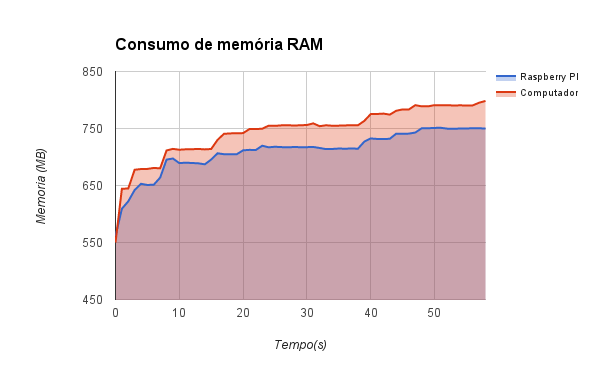
\includegraphics[scale=0.8]{Imagens/memoria}
\caption{Legenda}
\label{fig:memoria}
\end{figure}


Os dados apresentados no gráfico indicão que o Raspberry PI utilizou em quase todos os período do teste uma quantidade menor de memória RAM que o computador, ambos executados nas mesmas condições. Durante a coleta desses dados utilizando o Raspberry PI, o pico de memória foi de 751,2109 MB, enquanto o computador utilizou o teto de 798,3632 MB. Uma razoável diferença, levando em conta que o servidor antes de inciar os testes utilizava entre 561,1641 MB e 549,8554 MB. 

Os dados coletados sobre o  uso de CPU mostram uma alternância no período dos testes, onde o Raspberry PI apresentou um resultado mediano em relação ao computador. Na figura \ref{fig:cpu} mostra os dados de utilização de CPU durante os testes três e quatro.

\begin{figure}[!htb]
\centering
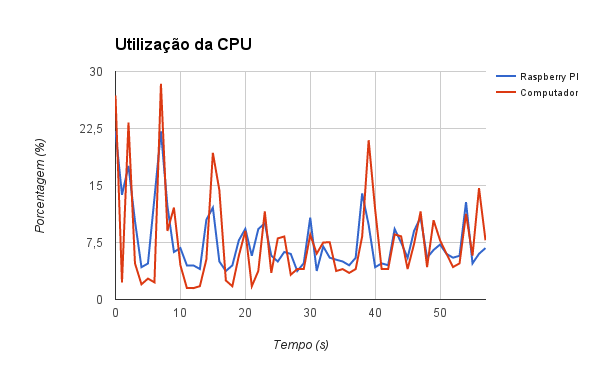
\includegraphics[scale=0.8]{Imagens/cpu}
\caption{Legenda}
\label{fig:cpu}
\end{figure}

A figura \ref{fig:cpu} mostra a utilização da CPU durante o período dos testes, onde é notado  uma alternância entre o computador e o Raspberry PI, no maior uso da CPU. O que indica um equilíbrio entre as ambas parte, já que a diferença é pequena do uso da CPU do servidor solicitada pelos thin clients  no mesmo instante do teste.
O ultima informação coletada dos testes está relacionado a transferência de dados pela rede, tendo em vista que para um melhor desempenho no ambente thin client, a rede local não pode ficar sobrecarregada. Foi coletado a quantidade de dados transferidos pela interface do servidor no instante de iniciou os testes e outra coleta após o tempo limite dos testes. Sendo assim possível verificar a quantidade de dados enviados e recebidos da interface do servidor usada para a comunicação com os thin clients.
Na figura \ref{fig:net} informa a quantidade de dados enviados e recebidos durante os testes. Lembrando que esses dados foram coletados do servidor.

\begin{figure}[!htb]
\centering
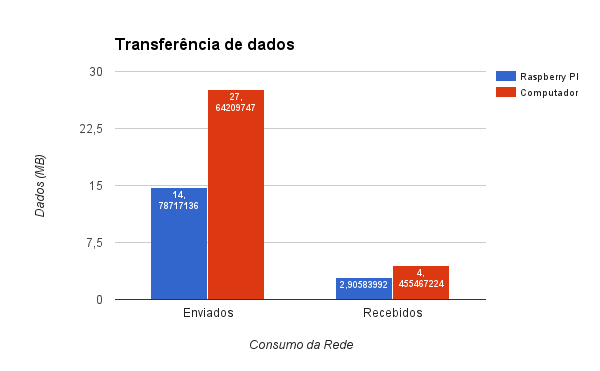
\includegraphics[scale=0.8]{Imagens/net}
\caption{Legenda}
\label{fig:net}
\end{figure}

O gráfico mostra bons resultados na utilização do Raspberry PI como thin client, necessitando apenas 14,78717136 MB de dados enviados  do servidor para executar os testes, isso é aproximadamente 53,47\% da quantidade solicitada pelo computador no modo thin client. Os resultados continuam favoráveis ao Raspberry PI nos dados que são enviados para o servidor, pois o ele enviou aproximadamente 65,21\% de dados que o computador executando o mesmo teste.

Os informações apresentadas na figura \ref{fig:net} indicam que a utilização de Raspberry PI no ambiente thin client torna a rede local mais “saudável”, transferindo menos dados e consequentemente ocupando menos largura de banda. 


% -----------------------------------------------------------------------------------------------------------
% Fim Análise e interpretação dos dados
% -----------------------------------------------------------------------------------------------------------

% -----------------------------------------------------------------------------------------------------------
% Finaliza o bookmark do PDF para que se inicie o bookmark na raiz e adiciona espaço de parte no Sumário
% -----------------------------------------------------------------------------------------------------------

\phantompart

% -----------------------------------------------------------------------------------------------------------
% Fim bookmark do PDF 
% -----------------------------------------------------------------------------------------------------------



% -----------------------------------------------------------------------------------------------------------
% Inseri Conclusão
% -----------------------------------------------------------------------------------------------------------

\part{Conclusão}

O Raspberry PI modelo B usando o BerryTerminal para ser um thin client, traz beneficios ao ambiente thin client, como a diminuição da utilização dos recursos do servidor, a economia de energia utilzada e a economia para criação de infraestrutura de computadores. A sua utilização se enquadra no conceito mais profundo do TI verde, ou Green IT, pois envolvendo uma nova estrutura de Refrigeração e um melhor aproveitamento dos espaços físicos. 

O Raspberry PI como um thin client, consome menos memória RAM que um computador com thin client, essa diferença em um ambiente com varias maquinas possibilita a inserção de mais Raspberrys PI do que computadores. Além de utilizar uma quantidade menor da banda em sua rede local.

Nos testes executados não foi possível acessar dispositivos de armazenamento conectado via usb no Raspberry PI, dificultando a transferência dos dados utilizados no ambiente thin client. E  uma das alternativa que viabiliza essa transferência é a conexão do dispositivo no servidor, algo que não é muito aconselhado e muitas vezes não é acessível aos usuário.

A usabilidade do Raspberry PI como thin client gerou resultados que não são motivos de elogio, já que ele teve um mal desempenho na execução de vídeos e dificuldades de na exibição da tela como a perda de algumas transições.

No geral, os resultados da comparação entre o computador e o Raspberry PI, ambos como thin client, foram neutros já que o Raspberry PI teve um melhor desempenho na utilização dos recursos e o computador desempenhou um ótimo papel usabilidade e na fluidez da utilização. deixando o placa equilibrado. Mas como o Raspberry PI possui outras vantagens como é preço e a sua economia de energia, tando diretamente quanto indiretamente. deixando o raspberry com um saldo positivo.

Então é correto afirma que o Raspberry PI é uma boa opção de thin client, mas vale ressaltar que é preciso verificar qual a finalidade do ambiente thin client, pois o Raspberry PI com o BerryTerminal não é aconselhado em ambientes onde ocorre edição de vídeos ou imagens. Mas altamente recomentado em ambientes onde se utiliza nuvens para o armazenamento dos dados.


% -----------------------------------------------------------------------------------------------------------
% Fim Conclusão
% -----------------------------------------------------------------------------------------------------------



% -----------------------------------------------------------------------------------------------------------
% ELEMENTOS PÓS-TEXTUAIS
% -----------------------------------------------------------------------------------------------------------

\postextual

% -----------------------------------------------------------------------------------------------------------
% Fim ELEMENTOS PÓS-TEXTUAIS
% -----------------------------------------------------------------------------------------------------------



% -----------------------------------------------------------------------------------------------------------
% Inseri Referências bibliográficas
% -----------------------------------------------------------------------------------------------------------

\bibliography{REFERENCIAS}

% -----------------------------------------------------------------------------------------------------------
% Fim Referências bibliográficas
% -----------------------------------------------------------------------------------------------------------

% ---
% Inicia os apêndices
% ---
\begin{apendicesenv}

% Imprime uma página indicando o início dos apêndices
\partapendices




\end{apendicesenv}
% ---


% ----------------------------------------------------------
% Anexos
% ----------------------------------------------------------

% ---
% Inicia os anexos
% ---
\begin{anexosenv}

% Imprime uma página indicando o início dos anexos
\partanexos

% ---

\end{anexosenv}

%---------------------------------------------------------------------
% INDICE REMISSIVO
%---------------------------------------------------------------------
\phantompart
\printindex
%---------------------------------------------------------------------

\end{document}
